\documentclass{beamer}
\usepackage[english]{babel}
\usepackage{amsmath}
\usepackage{graphicx}
\usepackage{lmodern}
\usepackage[font=small,format=plain,labelfont=bf,up,textfont=it,up]{caption}
\usepackage{url}
\usepackage{courier}
\usepackage[T1]{fontenc}
\usepackage{subcaption}
\usepackage{listings}
\usepackage{xcolor}
\usepackage[plain,vlined]{algorithm2e}

\setcounter{secnumdepth}{5}
\setlength{\parindent}{0in}

\usetheme{Antibes}
\setbeamertemplate{footline}[frame number]

\newcommand{\squeezeup}{\vspace{0mm}}

\renewcommand{\topfraction}{0.85}
\renewcommand{\textfraction}{0.1}
\renewcommand{\floatpagefraction}{0.75}

\definecolor{keyword}{RGB}{70,100,200}
\definecolor{kernel}{RGB}{139,0,0}
\definecolor{arrow}{RGB}{200,0,0}

\def\nese{\mathrel{%
    \mathchoice{\NESE}{\NESE}{\scriptsize\NESE}{\tiny\NESE}%
}}
\def\NESE{{%
    \setbox0\hbox{$\nearrow$}%
    \rlap{\hbox to \wd0{\hss $\searrow$ \hss}}\box0
}}

\def\nesecol{\mathrel{%
    \mathchoice{\NESECOL}{\NESECOL}{\scriptsize\NESECOL}{\tiny\NESECOL}%
}}
\def\NESECOL{{%
    \setbox0\hbox{$\nearrow$}%
    \rlap{\hbox to \wd0{\hss \textcolor{arrow}{$\searrow$} \hss}}\box0
}}

\def\nwsw{\mathrel{%
    \mathchoice{\NWSW}{\NWSW}{\scriptsize\NWSW}{\tiny\NWSW}%
}}
\def\NWSW{{%
    \setbox0\hbox{\textcolor{arrow}{$\nwarrow$}}%
    \rlap{\hbox to \wd0{\hss $\swarrow$ \hss}}\box0
}}

\newcommand\blfootnote[1]{%
  \begingroup
  \renewcommand\thefootnote{}\footnote{#1}%
  \addtocounter{footnote}{-1}%
  \endgroup
}

\title{Gene-Environment Interaction Analysis Using Graphic Cards}
\author{Daniel Berglund}
\date{17 February 2015}

\begin{document}

\begin{frame}
 \titlepage
\end{frame}

\section*{Outline}
\begin{frame}
\frametitle{Outline}
 \tableofcontents
\end{frame}

\section{Background}

\begin{frame}
\frametitle{Problem}

\begin{minipage}{0.5\textwidth}
\begin{itemize}
 \item Genetic and environmental factors are know to affect the risks of diseases
 \item Interaction can exist between these factors
\end{itemize}
\end{minipage}\hfill
\begin{minipage}{0.45\textwidth}
\begin{figure}[H]
\includegraphics[width=5.5cm]{ra_smoke_example.png}
\end{figure}
\end{minipage}

\blfootnote{Klareskog L, Stolt P, Lundberg K, et. al. A new model for an etiology of rheumatoid arthritis: smoking may trigger HLA-DR (shared epitope)-restricted immune reactions to autoantigens modified by citrullination. Arthritis Rheum 2006}

\end{frame}

\begin{frame}
\frametitle{Aim}
 
\begin{itemize}
 \item Data amounts are increasing, need for better programs
 \item GPUs have previously shown good results for gene-gene interaction
 \item Build a program for gene-environment interaction using GPUs based on older programs
\end{itemize}

\end{frame}

%TODO some genetics

%\begin{frame}
%\frametitle{The Data}
 
%\begin{itemize}
% \item The data consists of individuals, their status, environmental factor, SNPs and covariates
% \item A SNP is a genetic marker
% \item The environmental factor is something in the environment, for instance smoking
% \item Covariates are variables that needs to be adjusted for, for instance age
%\end{itemize}

%\end{frame}

\begin{frame}
\frametitle{Contingency Table}

%TODO �ndra till RA, covariates, gen+milj�
\begin{table}[h]
\centering
\begin{tabular}{| l c c c c c |}
  \hline
  & \multicolumn{2}{c}{Case} & & \multicolumn{2}{c}{Control}\\
  Genetic marker & A & B & & A & B\\
  \hline
  Smoker & 688 & 650 & & a & b\\
  Non smoker & 21 & 59 & & a & b\\
  \hline
\end{tabular}
\label{table:contingency_table}
\end{table}

\end{frame}

\begin{frame}
\frametitle{Relative Risk, Odds and Odds Ratio}

\begin{equation*}
RR=\frac{\pi_1}{\pi_2}
\end{equation*}

\begin{equation*}\label{eq:odds}
\Omega=\frac{\pi}{1-\pi}
\end{equation*}

\begin{equation*}\label{eq:odds_ratio}
OR=\frac{\Omega_1}{\Omega_2}
\end{equation*}

%\begin{equation*}
%\theta_{both\:factors\:present}>\theta_{first\:factor\:present}+\theta_{second\:factor\:present}-1
%\end{equation*}

\end{frame}

\begin{frame}
\frametitle{Logistic Regression}

\begin{equation*}
\log(\frac{\pi}{1-\pi})=\alpha+\beta X
\end{equation*}

\begin{equation*}
OR=e^{\beta}
\end{equation*}

$\beta$ coefficients can be found by using maximum likelihood

\end{frame}

\begin{frame}
\frametitle{Concurrency Architectures}
 \begin{figure}
        \centering
        \begin{subfigure}[b]{0.48\textwidth}
                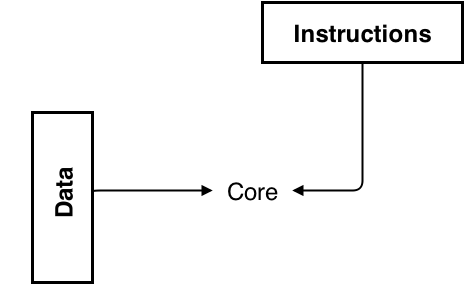
\includegraphics[width=3.5cm]{../SISD}
                \caption*{SISD}
        \end{subfigure}%
        ~
        \begin{subfigure}[b]{0.48\textwidth}
                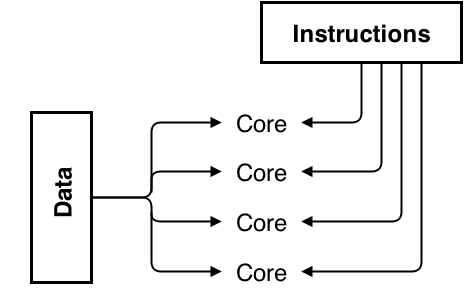
\includegraphics[width=3.5cm]{../MISD}
                \caption*{MISD}
        \end{subfigure}

        \begin{subfigure}[b]{0.48\textwidth}
                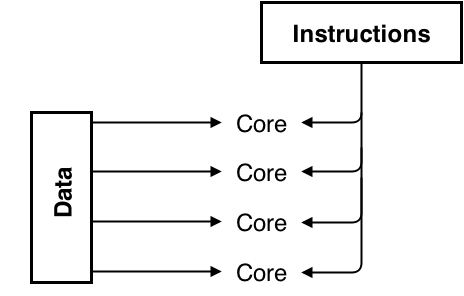
\includegraphics[width=3.5cm]{../SIMD}
                \caption*{SIMD}
        \end{subfigure}
        ~
        \begin{subfigure}[b]{0.48\textwidth}
                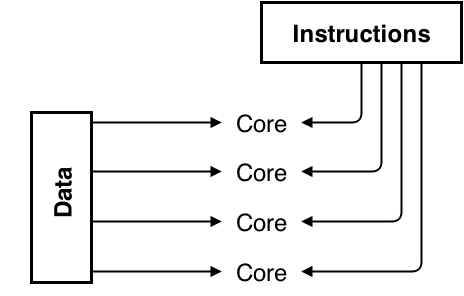
\includegraphics[width=3.5cm]{../MIMD}
                \caption*{MIMD}
        \end{subfigure}
\end{figure}
\end{frame}

%TODO CPU
\begin{frame}
\frametitle{CPU Architecture}

\begin{minipage}{0.5\textwidth}
\begin{itemize}
 \item MIMD
 \item 8 cores
 \item Lots of various optimizations
 \item 20 MB cache
 \item Similar performance with single and double precision
\end{itemize}
\end{minipage}\hfill
\begin{minipage}{0.45\textwidth}
\begin{figure}[H]
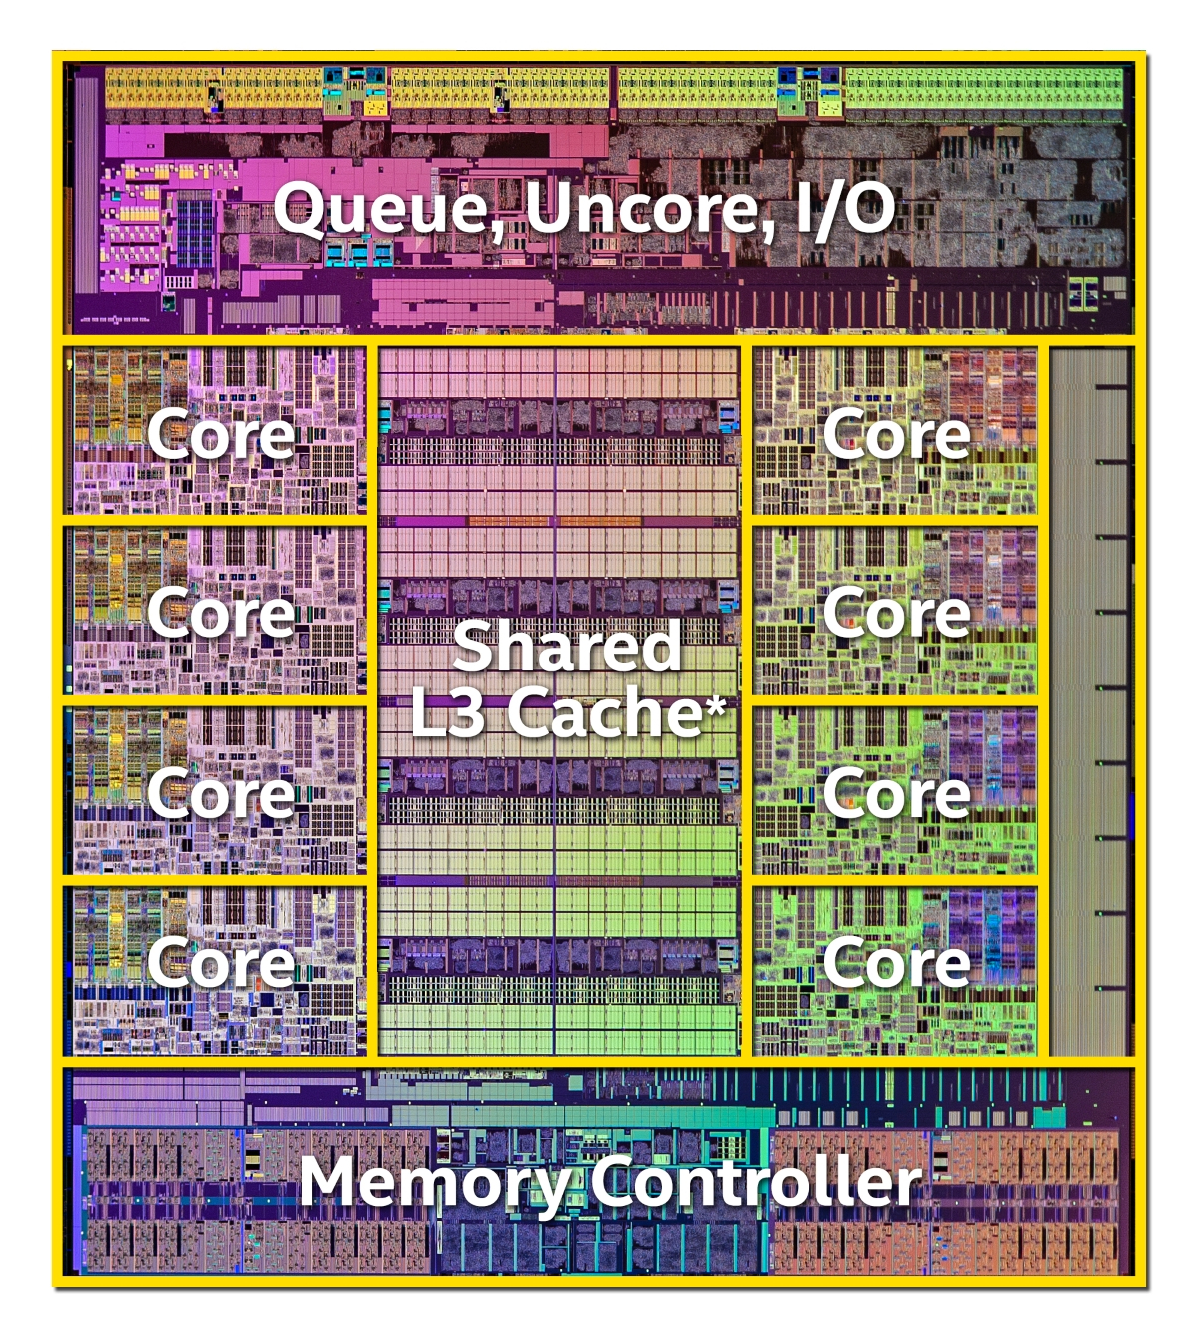
\includegraphics[width=4cm]{../cpu_scheme_haswell}
\end{figure}
\end{minipage}

\end{frame}

\begin{frame}
\frametitle{GPU Architecture}

\begin{figure}[h]
    \centering
    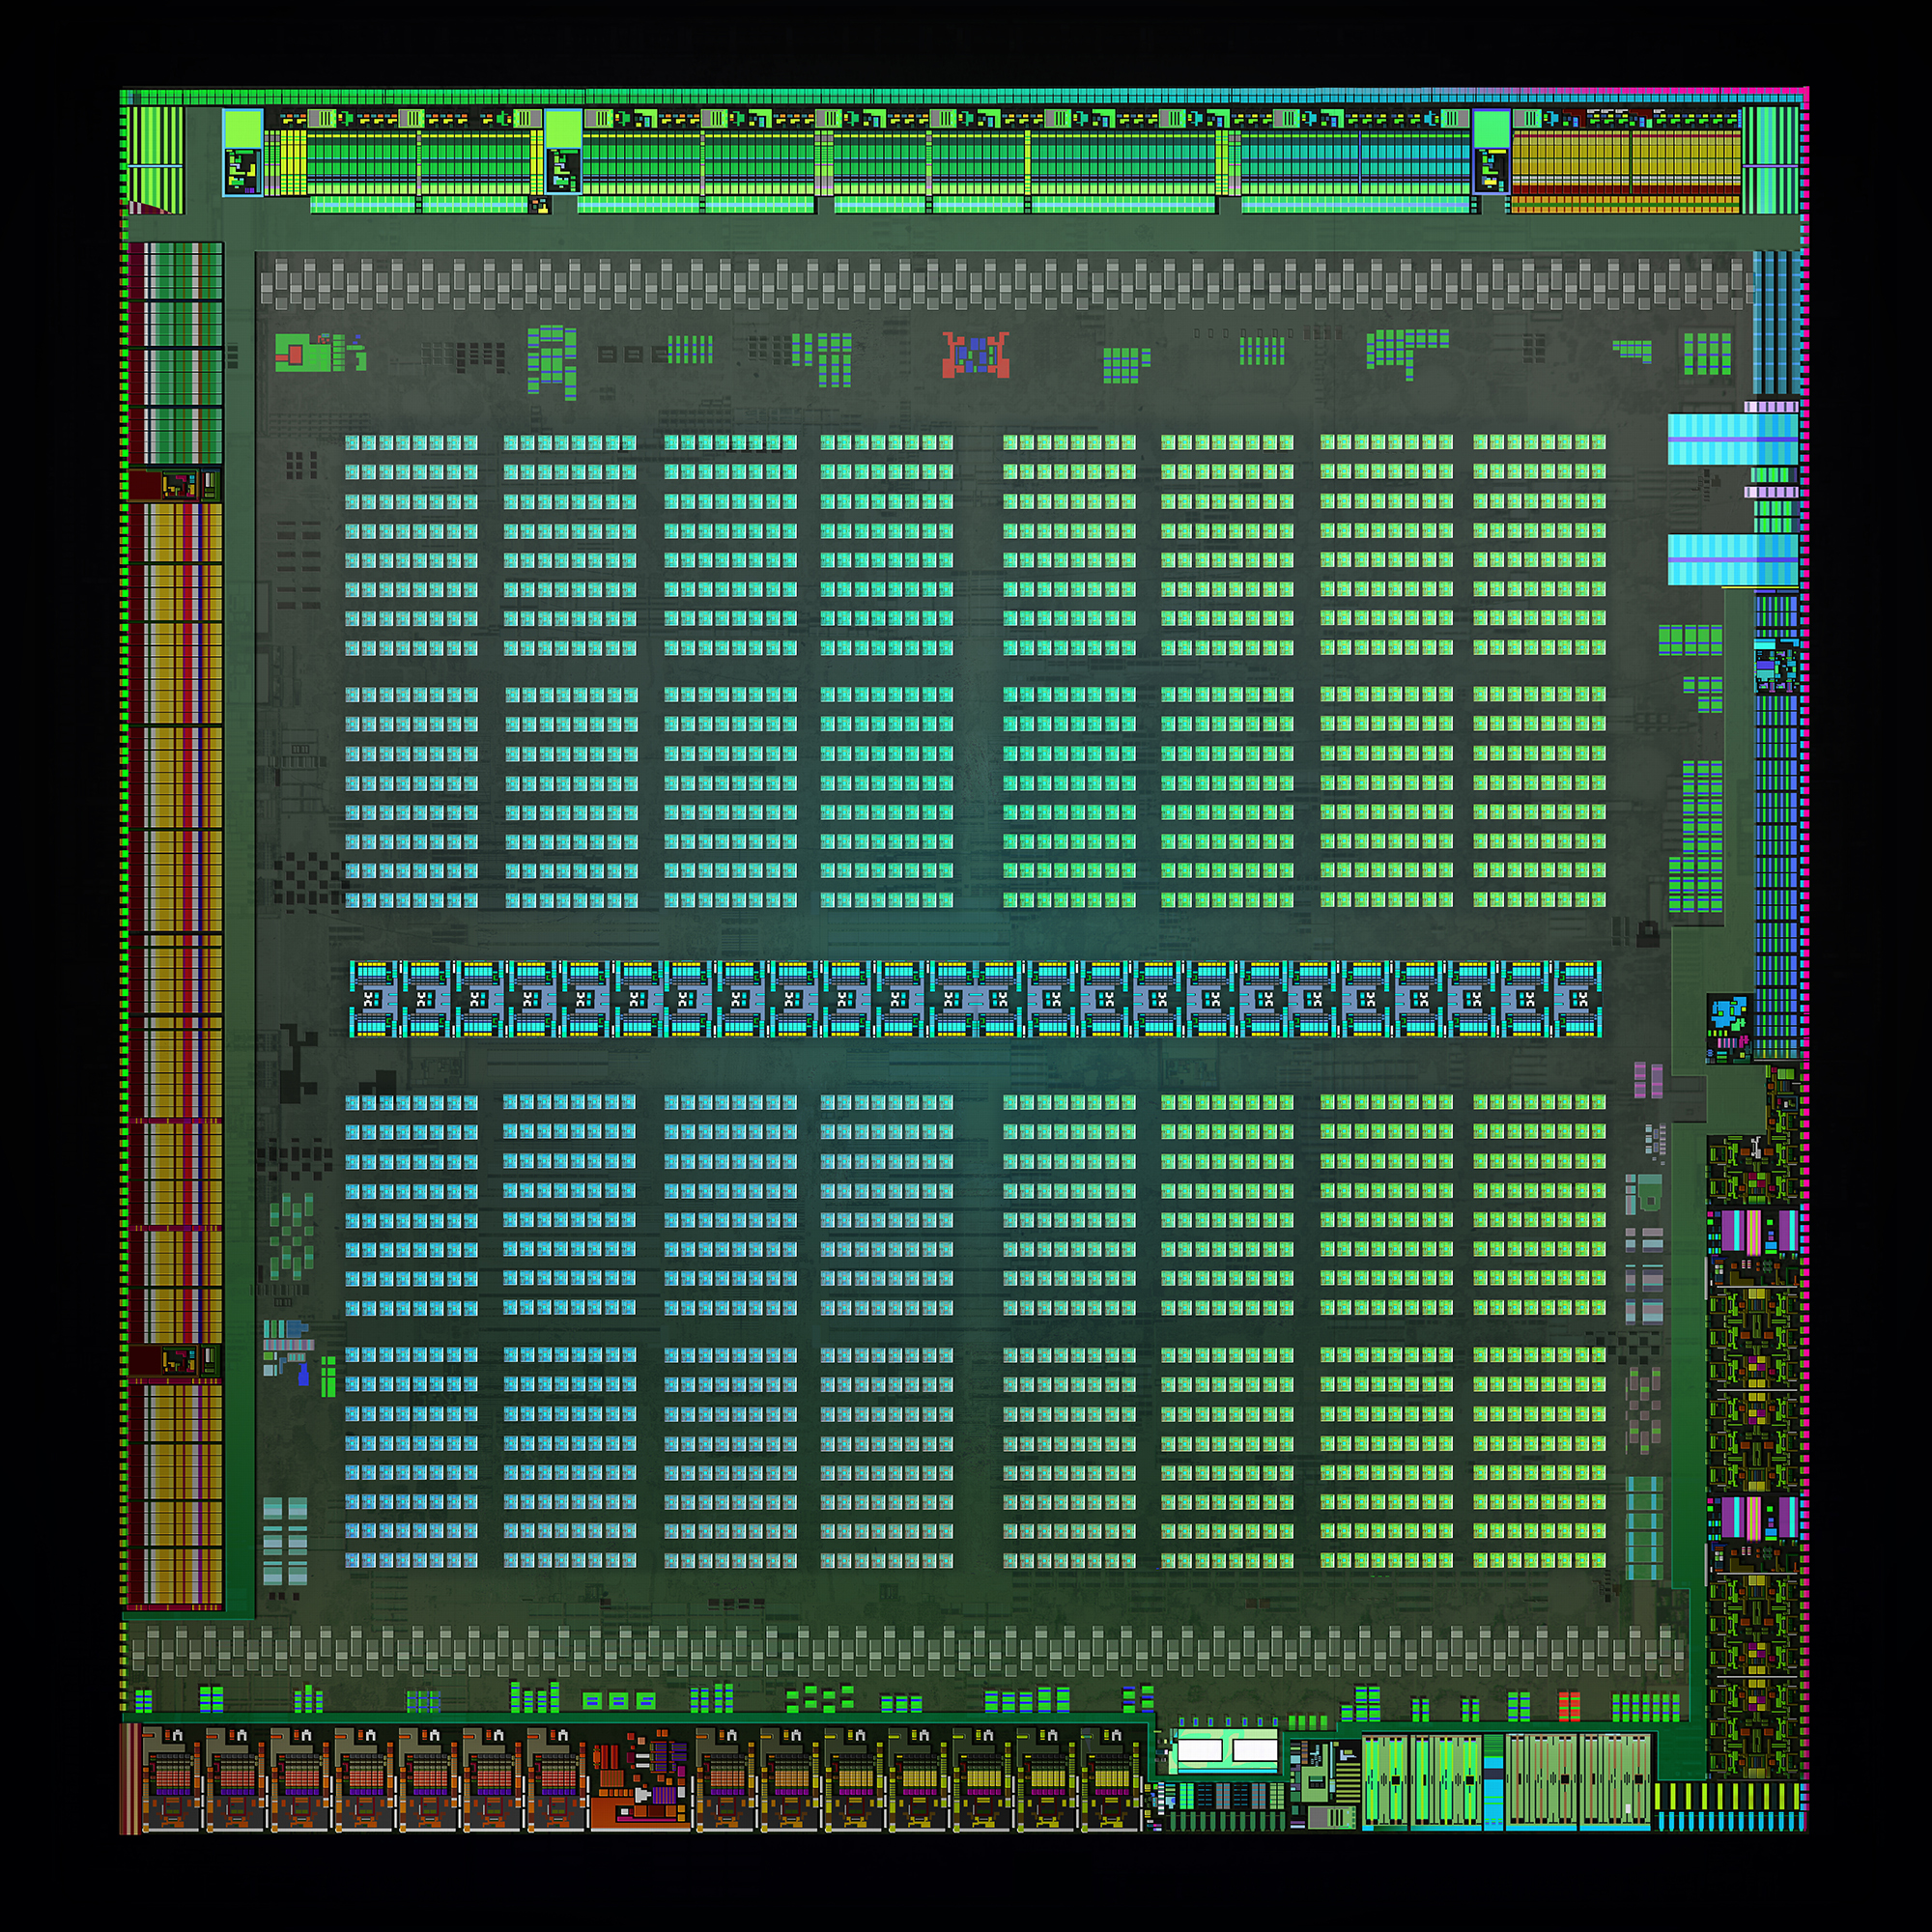
\includegraphics[width=6cm]{maxwell_die.jpg}
    \label{fig:gpu_scheme}
\end{figure}

\end{frame}

\begin{frame}
\frametitle{GPU Architecture}

\begin{itemize}
 \item Separate memory from the normal RAM
 \item Data has to be explicitly transferred to and from the GPU
 \item Fewer optimizations than CPU
 \item Slow but many cores, up to 5000
 \item Much better performance with single precision than double
 \item Single instruction, multiple thread(SIMT)
\end{itemize}

\end{frame}

%TODO cpu vs gpu
\begin{frame}
\frametitle{CPU versus GPU}

\begin{itemize}
 \item Pick tool based on the problem
 \item CPU for complex control flows
 \item GPUs need embarrassingly parallelism
 \item CPUs are becoming more like GPUs and vice versa
 \item Xeon Phi, CPU accelerators
\end{itemize}

\end{frame}

\begin{frame}
\frametitle{CUDA}

\begin{itemize}
 \item Compute Unified Device Architecture
 \item For NVIDIA GPUs by NVIDIA
 \item Supported by various libraries, for instance CUBLAS, Thrust
 \item Calculations done by kernels
\end{itemize}

\end{frame}

\begin{frame}
\frametitle{Kernel Example}

\begin{algorithm}[H]
\DontPrintSemicolon
\SetStartEndCondition{ (}{)}{)}\SetAlgoBlockMarkers{\{}{\}}
\SetKwProg{Fn}{}{}{}\SetKwFunction{FRecurs}{void FnRecursive}
\SetKwFor{For}{for}{}{}
\SetKwIF{If}{ElseIf}{Else}{if}{}{elif}{else}{}
\SetKwFor{While}{while}{}{}
\SetKwRepeat{Repeat}{repeat}{until}
\AlgoDisplayBlockMarkers
\SetAlgoNoLine
\SetFuncSty{}
\SetArgSty{}

\BlankLine \BlankLine

\SetKwFunction{KwFn}{\textcolor{kernel}{\_\_global\_\_} void \KwSty{Add}}

\Fn(){\KwFn{\textcolor{keyword}{float}* $A$, \textcolor{keyword}{float}* $B$, \textcolor{keyword}{float}* $C$}}{
\textcolor{keyword}{int} $i$ = threadIdx.$x$;\;
$C[i]$ = $A[i]$ $+$ $B[i]$;\;
}

\end{algorithm}

\begin{algorithm}[H]
\DontPrintSemicolon
\SetStartEndCondition{ (}{)}{)}\SetAlgoBlockMarkers{\{}{\}}%
\SetKwProg{Fn}{}{}{}\SetKwFunction{FRecurs}{void FnRecursive}%
\SetKwFor{For}{for}{}{}%
\SetKwIF{If}{ElseIf}{Else}{if}{}{elif}{else}{}%
\SetKwFor{While}{while}{}{}%
\SetKwRepeat{Repeat}{repeat}{until}%
\AlgoDisplayBlockMarkers\SetAlgoNoLine%

\BlankLine \BlankLine

\textbf{Add}\textcolor{kernel}{$<<<N$,$M>>>$}($A, B, C$);\;

\end{algorithm}

\end{frame}

\begin{frame}
\frametitle{Streams}

\begin{itemize}
 \item Kernels and transfers can be performed on streams
 \item Transfers and kernels can overlap when using streams
\end{itemize}

\end{frame}

\begin{frame}
\frametitle{Streams}

\begin{figure}[h]
    \centering
    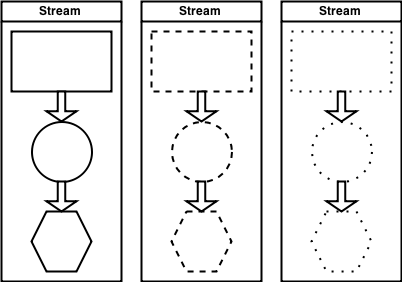
\includegraphics[width=7cm]{../StreamsQueue.png}
\end{figure}

\end{frame}

\begin{frame}
\frametitle{Streams}

\begin{figure}
        \centering
        \begin{subfigure}[b]{0.48\textwidth}
        \centering
                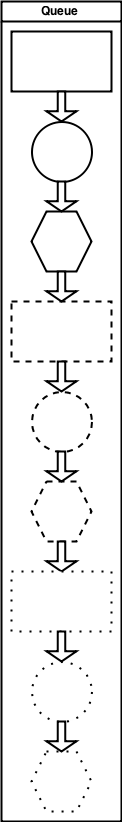
\includegraphics[width=0.9cm]{../StreamsQueueStreamLoop.png}
                \caption*{Looped over stream}
        \end{subfigure}%
        ~
        \begin{subfigure}[b]{0.48\textwidth}
        \centering
                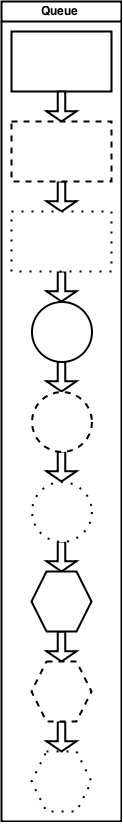
\includegraphics[width=0.9cm]{../StreamsQueueKernelLoop.png}
                \caption*{Looped over kernel}
        \end{subfigure}
\end{figure}

\end{frame}

\section{Implementation}

\begin{frame}
\frametitle{Agile Development}
\begin{itemize}
 \item Code in small units, commonly classes
 \item Unit testing, test the units in isolation
 \item Mocks, i.e. fake objects
 \item If a unit is working incorrectly only its corresponding unit test should fail
 \item Integration tests can be used to test if the units work properly together
\end{itemize}

\end{frame}

\begin{frame}
\frametitle{Wrappers}

\begin{itemize}
 \item Wrappers are used to ``fix'' interfaces
 \item Does not perform the task, delegates it
\end{itemize}

\end{frame}

\begin{frame}
\frametitle{Wrappers}

\begin{algorithm}[H]
\DontPrintSemicolon
\SetStartEndCondition{ (}{)}{)}\SetAlgoBlockMarkers{\{}{\}}%
\SetKwProg{Fn}{}{}{}\SetKwFunction{FRecurs}{void FnRecursive}%
\SetKwFor{For}{for}{}{}%
\SetKwIF{If}{ElseIf}{Else}{if}{}{elif}{else}{}%
\SetKwFor{While}{while}{}{}%
\SetKwRepeat{Repeat}{repeat}{until}%
\AlgoDisplayBlockMarkers\SetAlgoNoLine%

\textbf{cublasSgemv}($cublasHandle$, $transpose$, $m$, $n$, $\alpha$, $matrix$, $ld\_matrix$, $vector$, $inc\_vector$,
      $\beta$, $result$, $inc\_result$);

\end{algorithm}

\begin{algorithm}[H]
\DontPrintSemicolon
\SetStartEndCondition{ (}{)}{)}\SetAlgoBlockMarkers{\{}{\}}%
\SetKwProg{Fn}{}{}{}\SetKwFunction{FRecurs}{void FnRecursive}%
\SetKwFor{For}{for}{}{}%
\SetKwIF{If}{ElseIf}{Else}{if}{}{elif}{else}{}%
\SetKwFor{While}{while}{}{}%
\SetKwRepeat{Repeat}{repeat}{until}%
\AlgoDisplayBlockMarkers\SetAlgoNoLine%

\BlankLine \BlankLine

\textbf{matrixVectorMultiply}($matrix$, $vector$, $result$, $\alpha$, $\beta$);

\end{algorithm}

\end{frame}

\begin{frame}
\frametitle{Structure of Program}

\begin{itemize}
 \item Called CuEira
 \item Written in C++
 \item Libraries used are Google Test/Mock, Boost, CUDA, CUBLAS
 \item Modularised
 \item Almost full unit test coverage
 \item Handles each gene environment combination independently
 \item Some parts are done using CPU
\end{itemize}

\end{frame}

\begin{frame}
\frametitle{Overview}

\begin{figure}[h]
    \centering
    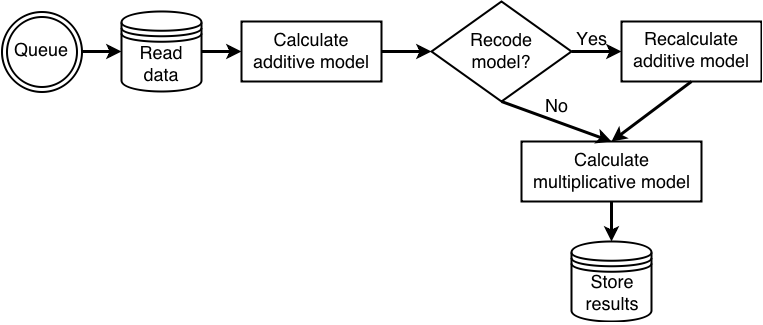
\includegraphics[width=10cm]{../SNP_thread.png}
\end{figure}

\end{frame}

\section{Results}

\begin{frame}
\frametitle{Data and Expectations}

\begin{itemize}
 \item Simulated data
 \item 10 000 SNPS
 \item 2000, 10 000, 100 000, 200 000 individuals
 \item 0, 5, 10, 20 covariates
 \item Expected linear efficiency
\end{itemize}

\end{frame}

\begin{frame}
\frametitle{Streams}

\begin{figure}[h]
    \centering
    \includegraphics[width=7cm]{../gpu_10streams_10ks_100ki.png}
\end{figure}

\end{frame}

\begin{frame}
\frametitle{Saturated Streams}

\begin{figure}[h]
    \centering
    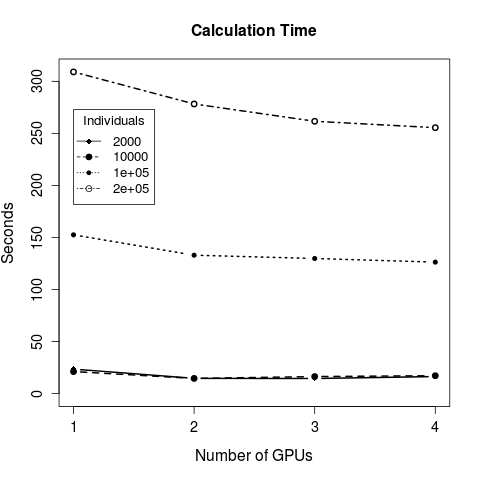
\includegraphics[width=6cm]{../saturated_gpu_seconds_ind_cov_0.png}
    \caption*{0 covariates}
\end{figure}

\end{frame}

\begin{frame}
\frametitle{Speedup and Efficiency}

Versus one GPU

\begin{figure}
        \centering
        \begin{subfigure}[b]{0.48\textwidth}
                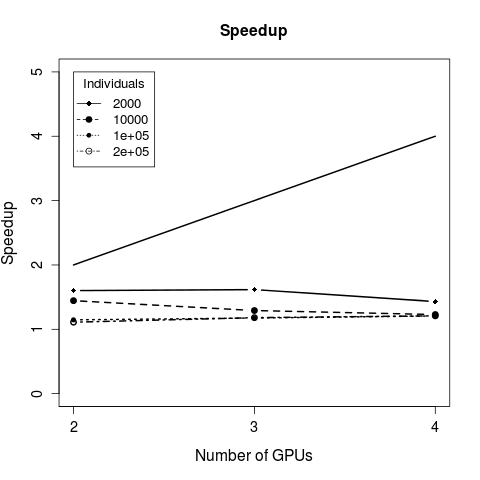
\includegraphics[width=5cm]{../saturated_gpu_speedup_ind_cov_0.png}
                \caption*{0 covariates}
        \end{subfigure}%
        ~
        \begin{subfigure}[b]{0.48\textwidth}
                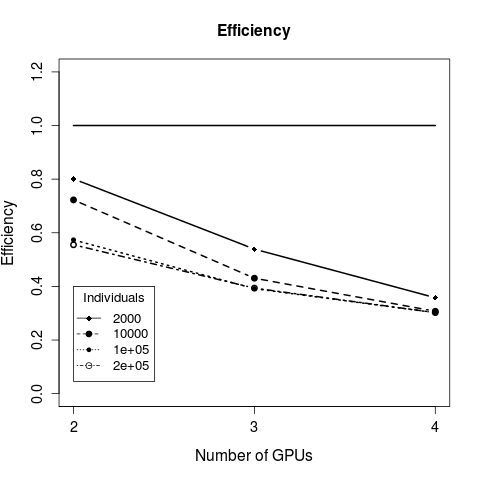
\includegraphics[width=5cm]{../saturated_gpu_efficiency_ind_cov_0.png}
                \caption*{0 covariates}
        \end{subfigure}
\end{figure}

\end{frame}

\begin{frame}
\frametitle{Single Versus Double Precision}

\begin{figure}
        \centering
        \begin{subfigure}[b]{0.48\textwidth}
        \centering
                \includegraphics[width=5cm]{../double_comp_cov_ind_10000.png}
                \caption*{10000 individuals}
        \end{subfigure}%
        ~
        \begin{subfigure}[b]{0.48\textwidth}
        \centering
                \includegraphics[width=5cm]{../double_comp_ind_cov_0.png}
                \caption*{0 covariates}
        \end{subfigure}
\end{figure}

\end{frame}

\begin{frame}
\frametitle{Synchronisation}

\begin{figure}
        \centering
        \begin{subfigure}[b]{0.48\textwidth}
                \includegraphics[width=5cm]{../sync_comp_cov_ind_2000.png}
                \caption*{2000 individuals}
        \end{subfigure}%
        ~
        \begin{subfigure}[b]{0.48\textwidth}
                \includegraphics[width=5cm]{../sync_comp_cov_ind_2e+05.png}
                \caption*{200 000 individuals}
        \end{subfigure}
\end{figure}

\end{frame}

\begin{frame}
\frametitle{Synchronisation}

\begin{figure}
        \centering
        \begin{subfigure}[b]{0.48\textwidth}
                \includegraphics[width=5cm]{../timedist_LR_ind_10ks_0cov_gpu4.png}
                \caption*{Less synchronisation}
        \end{subfigure}%
        ~
        \begin{subfigure}[b]{0.48\textwidth}
                \includegraphics[width=5cm]{../timedist_LR_ind_10ks_0cov_gpu4_sync.png}
                \caption*{Always synchronise}
        \end{subfigure}
\end{figure}

\end{frame}

\begin{frame}
\frametitle{Comparison versus GEISA}

\begin{figure}
        \centering
        \begin{subfigure}[b]{0.48\textwidth}
                \includegraphics[width=5cm]{../geisa_saturated_speedup_ind.png}
                \caption*{0 covariates}
        \end{subfigure}%
        ~
        \begin{subfigure}[b]{0.48\textwidth}
                \includegraphics[width=5cm]{../geisa_saturated_speedup_cov.png}
                \caption*{10 000 individuals}
        \end{subfigure}
\end{figure}

\end{frame}

\section{Conclusions and Outlook}

\begin{frame}
\frametitle{Conclusions}

\begin{itemize}
 \item GPUs suits well for interaction, depending on method
 \item Use one, perhaps two, GPUs with the program
 \item Single precision gives better performance than double precision
 \item Increased synchronisation increases performance slightly when number of individuals is above 100 000
\end{itemize}

\end{frame}

\begin{frame}
\frametitle{Outlook}

\begin{itemize}
 \item Implement a method for validation, bootstrap or permutation tests
 \item Moving more parts to the GPU could fix the bad scaling
 \item Clusters for more speed
 \item Need for better statistics and definitions of interaction for non binary factors
 \item For binary factors look into gene-gene interaction methods if further speed is needed
\end{itemize}

\end{frame}

%TODO 
\begin{frame}
%\frametitle{GPU Architecture}

Thanks to:\\

CuEira is available at:
github.com/Berjiz/CuEira

\end{frame}

\begin{frame}
\frametitle{CPU versus GPU}

\begin{table}[h]
\centering
\begin{tabular}{| l | c | c | c |}
  \hline
   & CPU & MIC & GPU\\
  \hline
  Example & Intel i7-5960X & Xeon Phi 7120A & K80\\
  \hline
  Cores & 8 & 61 & 4992\\
  Memory & 0.1-1 TB & 16GB & 24 GB\\
  Caches & 20 MB & 30.5 MB & -\\
  Concurrency & MIMD & MIMD & SIMT\\
  FLOPS & 0.4 T & 3 T & 3, 8.7 T \\
  Price & \$1000 & \$4200 & \$5000\\
  \hline  
\end{tabular}
\end{table}

\end{frame}

\begin{frame}
\frametitle{Matrix Decomposition}

\begin{itemize}
 \item Pseudo inverse, $A^+$, is defined for general matrices
 \item Can be found by using singular value decomposition
\end{itemize}

\begin{equation*}
A=U \Sigma V^T
\end{equation*}

\begin{equation*}
A^+=V \Sigma^+ U^T
\end{equation*}

\end{frame}

\begin{frame}
\frametitle{Recoding}

\begin{itemize}
 \item The measures for additive interaction are defined for positive odds ratios
 \item Can be adjusted by recoding
 \item Recoding switches the reference group with the group with lowest risks
 \item Guarantees that $OR \geq 1$
\end{itemize}

\end{frame}

\begin{frame}
\frametitle{Speedup and Efficiency}

\begin{equation*}
S(p)=\frac{T(1)}{T(p)}
\end{equation*}

\begin{equation*}
E(p)=\frac{S(p)}{p}=\frac{T(1)}{pT(p)}
\end{equation*}

\end{frame}

\begin{frame}
\frametitle{Concurrency and Dinning Philosophers}

\begin{figure}[h]
    \centering
    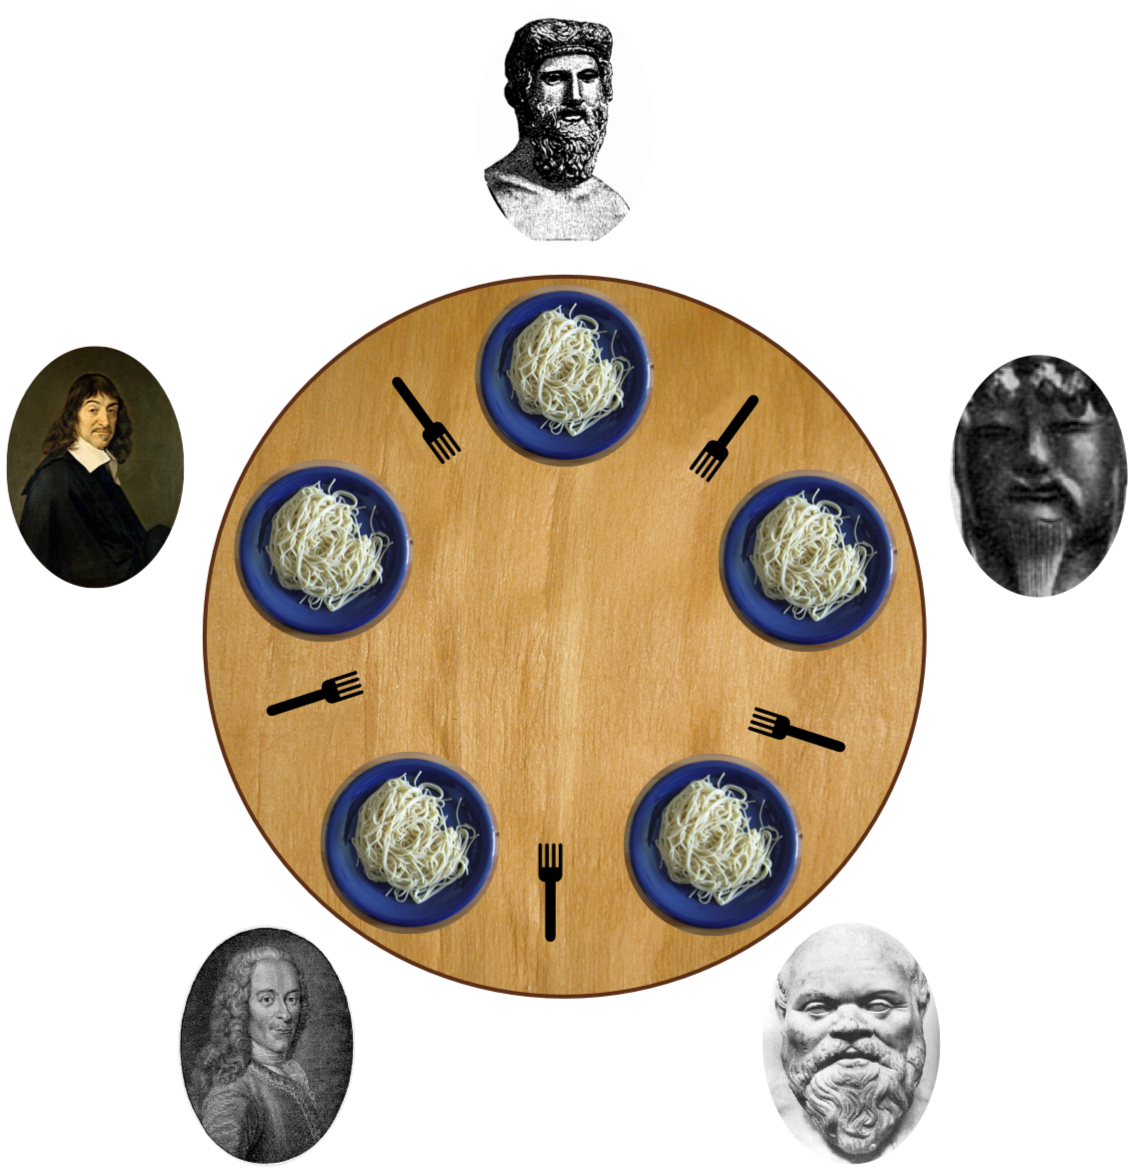
\includegraphics[width=5cm]{../dining_philosophers.png}
\end{figure}

\end{frame}

\begin{frame}
\frametitle{A Possible Solution} 

\begin{itemize}
 \item Think
 \item Wait for a fork to become available and pick up that fork
 \item Wait for and pick up the other fork
 \item Eat
 \item Put down the forks one by one
 \item Go back to thinking
\end{itemize}

\end{frame}

\begin{frame}
\frametitle{Deadlock}

\begin{itemize}
 \item Stuck when everyone holds one fork
 \item This is a deadlock
 \item Can be solved with a mediator
\end{itemize}

\end{frame}

\begin{frame}
\frametitle{Time Distribution for Kernels}

{\tiny $*$ is element by element multiplication}

\squeezeup

\begin{table}[h]
\centering
\begin{tabular}{| l | l | c | c | c | c |}
  \hline
  Covariates & & 0 & 0 & 20 & 20 \\
  Individuals & & 10k & 100k & 10k  & 100k  \\
  \hline
  $M1^T \cdot V1$ & CUBLAS & 66.6 & 72.2 & 43 & 53.9\\
  $M1 \cdot M2$ & CUBLAS & 18.9 & 14.4 & 36.1 & 25.8\\
  $M1 \cdot V1$ & CUBLAS & 7.1 & 8.1 & 5.9 & 7.4\\
  $V1 * V2$ & Custom & 2.9 & 2.3 & 11.8 & 10.6\\
  $\frac{e^{V1}}{1+e^{V1}}$ & Custom & 1.1 & 0.9 & 0.7 & 0.7\\
  %$V1*\log(V2)+$ \newline $(1-V1)*\log(1-V2)$
  
{$\begin{aligned}
& V1*\log(V2)+\\
& (1-V1)*\log(1-V2)
\end{aligned}$}
  & Custom & 0.8 & 0.6 & 0.6 & 0.5\\
    
  $V1 - V2$ & Custom & 0.7 & 0.6 & 0.5 & 0.4\\
  $V1*(1-V1)$ & Custom & 0.7 & 0.5 & 0.4 & 0.4\\
  \emph{Dot product} & CUBLAS & 0.7 & 0.3 & 0.3 & 0.2\\
  $\Sigma V1$ & CUBLAS & 0.5 & 0.1 & 0.2 & 0.1\\
  \hline  
\end{tabular}
\end{table}

\end{frame}

\begin{frame}
\frametitle{Blocks}

\begin{figure}[h]
    \centering
    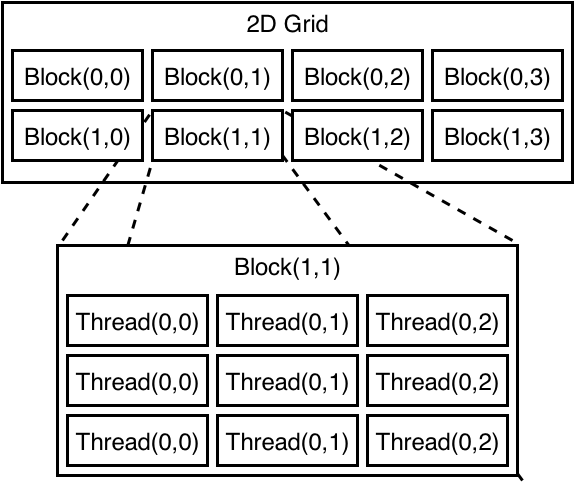
\includegraphics[width=7cm]{../2D_grid.png}
\end{figure}

\end{frame}

\begin{frame}
\frametitle{Blocks}

\begin{figure}[h]
    \centering
    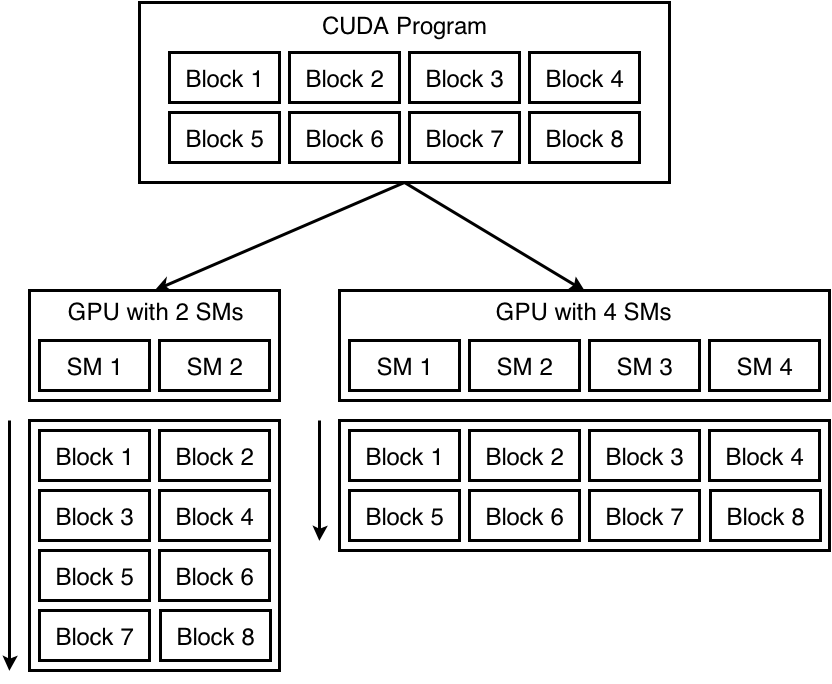
\includegraphics[width=7cm]{../grid_scale.png}
\end{figure}

\end{frame}

%TODO make slides about possible questions

%opencl vs cuda

\end{document}